% Template for Cogsci submission with R Markdown

% Stuff changed from original Markdown PLOS Template
\documentclass[10pt, letterpaper]{article}

\usepackage{cogsci}
\usepackage{pslatex}
\usepackage{float}
\usepackage{caption}

% amsmath package, useful for mathematical formulas
\usepackage{amsmath}

% amssymb package, useful for mathematical symbols
\usepackage{amssymb}

% hyperref package, useful for hyperlinks
\usepackage{hyperref}

% graphicx package, useful for including eps and pdf graphics
% include graphics with the command \includegraphics
\usepackage{graphicx}

% Sweave(-like)
\usepackage{fancyvrb}
\DefineVerbatimEnvironment{Sinput}{Verbatim}{fontshape=sl}
\DefineVerbatimEnvironment{Soutput}{Verbatim}{}
\DefineVerbatimEnvironment{Scode}{Verbatim}{fontshape=sl}
\newenvironment{Schunk}{}{}
\DefineVerbatimEnvironment{Code}{Verbatim}{}
\DefineVerbatimEnvironment{CodeInput}{Verbatim}{fontshape=sl}
\DefineVerbatimEnvironment{CodeOutput}{Verbatim}{}
\newenvironment{CodeChunk}{}{}

% cite package, to clean up citations in the main text. Do not remove.
\usepackage{cite}

\usepackage{color}

% Use doublespacing - comment out for single spacing
%\usepackage{setspace}
%\doublespacing


% % Text layout
% \topmargin 0.0cm
% \oddsidemargin 0.5cm
% \evensidemargin 0.5cm
% \textwidth 16cm
% \textheight 21cm

\title{Exploring a Causal Link between Language and Cultural Biases}


\author{{\large \bf Molly Lewis} \\ \texttt{mollyllewis@gmail.com} \\ Department of Psychology  \\ University of Wisconsin-Madison \And {\large \bf Gary Lupyan} \\ \texttt{lupyan@wisc.edu} \\ Department of Psychology  \\ University of Wisconsin-Madison}

\begin{document}

\maketitle

\begin{abstract}
The abstract.

\textbf{Keywords:}
IAT, cultural biases, gender, linguistic relativity.
\end{abstract}

\section{Introduction}\label{introduction}

\section{Study 1: Measuring cross-cultural gender
bias}\label{study-1-measuring-cross-cultural-gender-bias}

\subsection{Method}\label{method}

We quantified the degree of gender bias in a culture using data from the
Implicit Association Task (``IAT''; (Greenwald, McGhee, \& Schwartz,
1998)). The IAT measures respondents' automatic associations between two
sets of concepts (e.g., male-career/female-family
vs.~male-family/female-career). The underlying assumption of the measure
is that concepts that are represented as more similar to each other in
the cognitive system should be easier to pair together in a behavioral
task, compared to two concepts that are relatively dissimilar. Concepts
are paired in the task by assigning them to the same response keys in a
2AFC categorization task. In the critical blocks of the task, concepts
are assigned to keys in a way that is either bias-congruent (i.e.~Key A
= male or career; Key B = female or family) or bias-incongruent
(i.e.~Key A = male or family; Key B = female or career). Participants
are then presented with a word related to one of the four concepts and
asked to classify it by responding with one of the two keys as quickly
as possible. Slower reaction times in the bias-incongruent blocks
relative to the bias-congruent blocks suggests an implicit association
between the two sets of concepts (i.e.~a bias to associate male with
career, and female with family). In the present study, we analyzed an
exisiting dataset of IAT scores collected online from a large,
culturally diverse sample (Project Implicit:
\url{https://implicit.harvard.edu/implicit/}; (Nosek, Banaji, \&
Greenwald, 2002)).

\subsection{Analysis}\label{analysis}

We analalyzed all gender IAT scores collected from respondents between
2005 and 2016 who had complete data and were located in countries with
more than 400 total respondents (\emph{N} = 773,205). We further
restricted our sample based on participants' reaction times and errors
using the same criteria described in Nosek, Banjai, and Greenwald (2002,
pg. 104). Our final sample included 664,359 participants from 49
countries, with a median of 1,123 participants per country.

Several measures have been used in the literature to describe the
difference in reaction time between bias congruent and incongruent
blocks (Greenwald, Nosek, \& Banaji, 2003). Here, we use the best
performing measure of implicit bias, ``D-score,'' which quantifies the
difference between critical blocks while also accounting for individual
differences in response time

In addition to an implicit measure, we also analyzed an explicit measure
of gender bias. After completing the IAT, participants were asked, ``How
strongly do you associate the following with males and females?'' for
both career and family. They indicated their response on a Likert scale
ranging from female (1) to male (7). We calculated an explicit gender
bias score for each participant as the career response minus the family
response, such that greater values indicated more gender bias as for the
D-score.

\subsection{Results}\label{results}

\begin{CodeChunk}
\begin{figure}[t]

{\centering 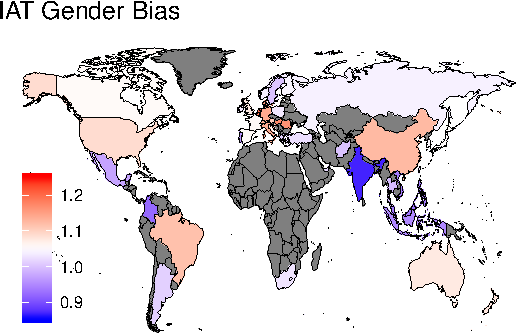
\includegraphics{figs/map-1} 

}

\caption[IAT gender bias (D-score) for the 49 countries with available data]{IAT gender bias (D-score) for the 49 countries with available data. All countries show a positive bias, with red indicating above average and blue indicating below average bias.}\label{fig:map}
\end{figure}
\end{CodeChunk}

Broadly, we replicate the previous pattern of findings on the gender IAT
(Nosek et al., 2002). First, participants in all countries showed bias
to associate men with career and females with family. Figure 1 shows the
magnitude of the IAT gender bias (D-score) across all 49 countries (M =
0.37; SD = 0.03). Second, implicit and explicit measures bias were
correlated both at the level of individual participants (\emph{r} =
0.15; \emph{p} \textless{} .00001) and at the level of countries
(\emph{r} = 0.31; \emph{p} = 0.03).

Finally, previous work has shown a difference for women

\subsection{Study 2a: Caliskan
replication}\label{study-2a-caliskan-replication}

\subsection{Study 2b: predicting implicit bias with language
iat}\label{study-2b-predicting-implicit-bias-with-language-iat}

\section{Study 3: grammar and bias}\label{study-3-grammar-and-bias}

\section{Study 4: exploring bias more
directly}\label{study-4-exploring-bias-more-directly}

\section{Conclusion}\label{conclusion}

\section{References}\label{references}

\setlength{\parindent}{-0.1in} \setlength{\leftskip}{0.125in} \noindent

\hypertarget{refs}{}
\hypertarget{ref-greenwald1998measuring}{}
Greenwald, A. G., McGhee, D. E., \& Schwartz, J. L. (1998). Measuring
individual differences in implicit cognition: The implicit association
test. \emph{Journal of Personality and Social Psychology}, \emph{74}(6),
1464.

\hypertarget{ref-greenwald2003understanding}{}
Greenwald, A. G., Nosek, B. A., \& Banaji, M. R. (2003). Understanding
and using the implicit association test: I. an improved scoring
algorithm. \emph{Journal of Personality and Social Psychology},
\emph{85}(2), 197.

\hypertarget{ref-nosek2002harvesting}{}
Nosek, B. A., Banaji, M. R., \& Greenwald, A. G. (2002). Harvesting
implicit group attitudes and beliefs from a demonstration web site.
\emph{Group Dynamics: Theory, Research, and Practice}, \emph{6}(1), 101.

\end{document}
